\begin{frame}
    \frametitle{Mathematical Analysis}

    
    \begin{itemize}
        \item We look into some of the properties of the algorithm, how it performs on a three-ary complete tree.\pause[]
        \item We'll analyse a upper-bound on the number of colors used in the graph, and a bound on the number of nodes are colored by certain color.
    \end{itemize} 
\end{frame}

\begin{frame}
    \frametitle{Total color upper bound}

    We need to prove a upper bound on the number of colors used by our algorithm.    

\end{frame}

\begin{frame}
    \frametitle{Total color upper bound}

    To prove this if we could prove how many nodes are colored by each of the colors (or their upper bound) then we can count the total number of colors used by the algorithm.    

\end{frame}


\begin{frame}
    \frametitle{Theoretical Bounds}

    \textit{First we analyze the number of nodes colored with color $1$.}
\end{frame}

\begin{frame}
    \frametitle{Number of Nodes with Color 1}

    \begin{align*}
        \frac{\textsf{Total Color 1 Nodes}}{\textsf{Total Nodes}} &= \frac{3^{x} + 3^{x - 2} + 3^{x-4} + \dots 3^{1}}{\displaystyle\sum_{i = 0} ^{i = x} 3^i}\\
    \end{align*}

    \textit{If number of layers is odd ($x$ is odd) then the upper part of the fraction stops at $1$ and $0$ otherwise.}

\end{frame}

\begin{frame}
    \frametitle{Number of Nodes with Color 1}

    \begin{align*}
        \textsf{Ratio of Color 1 node to total nodes} &= \frac{3^{x} + 3^{x - 2} + 3^{x-4} + \dots 3^{1}}{\displaystyle\sum_{i = 0} ^{i = x} 3^i}\\
        &= \frac{3 \cdot \frac{9^{\frac{x}{2}} - 1}{9 - 1}}{\frac{3^x - 1}{2}}\\
        &= \frac{3}{4} \cdot \frac{3^x - 1}{3^x - 1}\\
        &= \frac{3}{4}
    \end{align*}    

\end{frame}

\begin{frame}
    \frametitle{Number of Nodes with Color 1}

    \begin{Fact}{Total Nodes with color 1}{}
        For complete trees we can color at most $\frac{3}{4}$ many nodes with color 1.
    \end{Fact}

\end{frame}

\begin{frame}
    \frametitle{Number of Nodes with Color 2}

    To count how many nodes are colored with color $2$ we'll approach this problem inductively.    

\end{frame}

\begin{frame}
    \frametitle{Number of nodes with color 2}


    \begin{itemize}
        \item First we find out for small size trees (for example level $3$ trees) how many nodes are colored with color $2$.\pause[]
        \item Then we extrapolate this to bigger trees. This analysis holds because bigger complete tree has these smaller complete threes as their children.
    \end{itemize}

\end{frame}

\begin{frame}
    \frametitle{Number of nodes with color 2}

    \begin{figure}
        \centering
        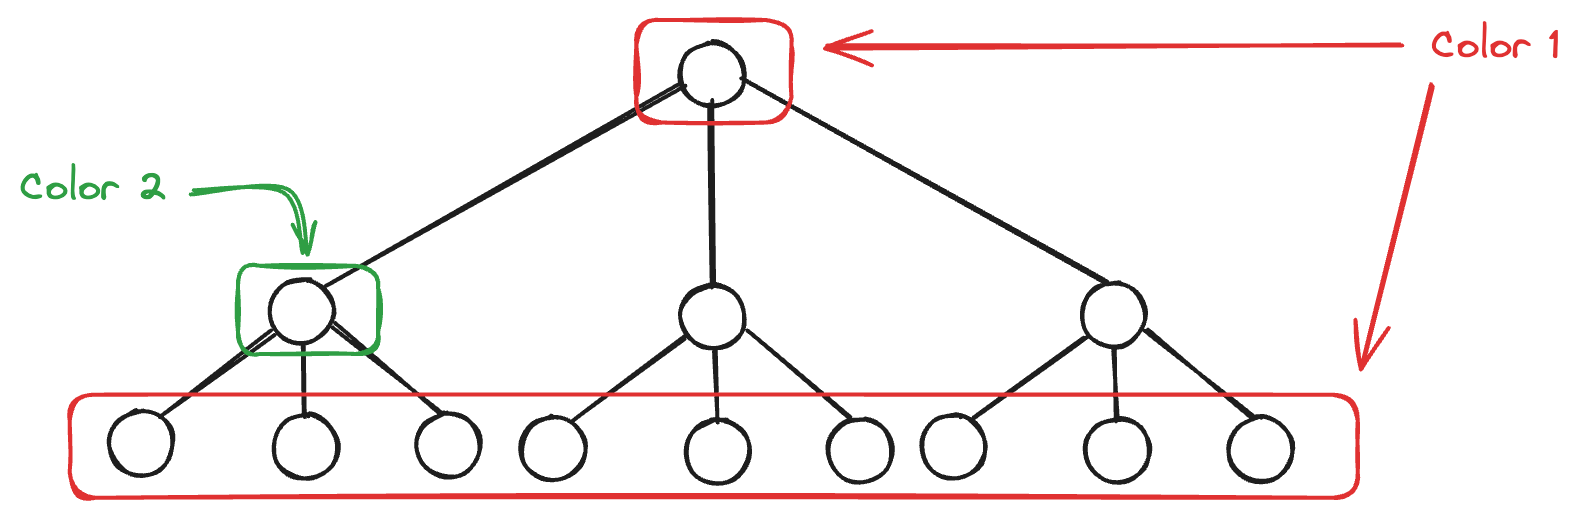
\includegraphics[width=0.7\linewidth]{images/layer 3.png}
        \caption{For a three layer deep tree only one node can be colored with Color $2$}
        \label{fig:enter-label}
    \end{figure}

\end{frame}

\begin{frame}
    \frametitle{Number of nodes with color 2}

    So for a four layer tree, the total number of nodes colored with color $2$ is $3 \times 1 = 3$

\end{frame}


\begin{frame}
    \frametitle{Number of nodes with color 2}

    \begin{itemize}
        \item Layer $4$ tree is a combination of $3$ layer $3$ trees connected with one extra node.\pause[]
        \item This extra node can not be colored with color $2$. Hence total color $2$ needed is three times the total color $2$ in the $3$ layered tree.    
    \end{itemize}

\end{frame}

\begin{frame}

    \frametitle{Number of nodes with color 2}
    
    
    \begin{itemize}
        \item Same thing is true for layer $5$ tree also because the extra node (top most node) here will be colored with color $1$ as odd layers are colored with color $1$.\pause[]
        \item At layer $6$ the top most node can be colored with color $2$. Hence for layer six the number of node is one more of $3$ times the number of nodes colored in layer $5$ tree.\pause[]
        \item We see a deviation from this pattern in layer $7$ tree.
    \end{itemize}

\end{frame}

\begin{frame}
    \frametitle{Layer 6 Trees}

    
    \begin{itemize}
        \item In layer $6$ tree we have $3$ layer $5$ trees connected with one extra node. The top most node is colored with color $2$\pause[]
        \item Each of the layer $6$ tree has $28$ nodes colored with color $2$.\pause[]
        \item However we can not combine these three layer $6$ trees with one extra node. Because the top most node in the layer $6$ colored with color $2$ will violate the distance conditions in the layer $7$ tree.\pause[]
        \item So we can only have one of the children (layer $6$) with color $2$ and rest are not colored with color $2$.\pause[]
        \item Hence we need to subtract $2$ from three times the total number of nodes colored with color $2$ in layer $6$ tree to count color $2$ nodes in layer $7$ trees.
    \end{itemize}

\end{frame}

\begin{frame}
    \frametitle{Generalization}

    Extending this concept to larger and larger trees we can see a pattern.
    
    \pause[]

    \begin{align*}
        A &= [0, 0, 1, -2]\\
        f_2(x) &= A[x \% 4] + 3 \cdot f_2(x - 1)
    \end{align*}


    \pause[]

    We use $f_2(3) = 1$ as the base-case. 

\end{frame}

\begin{frame}
    \frametitle{Approximation of number of nodes colored with color $2$}

    \begin{lemm}{Color $2$ node count}{}
        Simple greedy heuristic for complete tree packing coloring, colors roughly $\frac{1}{10} ^{\text{th}}$ many nodes with color $2$ as compared to color $1$.
    \end{lemm}

\end{frame}

\begin{frame}
    \frametitle{Proof}

    \begin{hypothesis}{}{}
        Suppose $f_2(x - 1) \approx \frac{1}{10} \cdot \frac{3}{4} \cdot \displaystyle\sum_{i = 0} ^{x - 2} 3^i$ is the number of color $2$ used by our algorithm for a $x - 1$ layer deep tree. 
    \end{hypothesis}

    We need to prove $f_2(x) \approx \frac{1}{10} \cdot \frac{3}{4} \cdot \displaystyle\sum_{i = 0} ^{x - 1} 3^i$ and verify this with experimental results.
\end{frame}

\begin{frame}
    \frametitle{Proof Continued}

    Using induction hypothesis and previous results we get,
    \begin{align*}
        f_2(x) &= A[x\%4] + 3 \cdot f_2(x - 1)\\
        &= A[x\%4] + 3 \cdot \frac{1}{10} \cdot \frac{3}{4} \cdot \displaystyle\sum_{i = 0} ^{x - 2} 3^i\\
        &= A[x\%4] + \frac{3}{4} \cdot \frac{1}{10} \cdot \displaystyle\sum_{i = 0} ^{x - 1} 3^i\\
        &\approx \frac{1}{10} f_1(x)
    \end{align*}

    Here $A[i] \in \{-2, 0, 1\}$, hence $f_2(x)$ is roughly $\frac{1}{10} \cdot f_1(x)$ where $f_1(x)$ is the number of color $1$ used.    

\end{frame}

\begin{frame}
    \frametitle{Results for other colors}

    We can also use these similar arguments for other higher colors, with that we can say the following facts\pause[]
    
    \begin{itemize}
        \item For three-ary complete trees number of nodes colored with color $(2, 3), (4, 5), (6, 7), \dots$ are the same pairwise,\pause[]
        \item For three-ary complete trees number of nodes colored with color $(4, 5),$ is one-third of the number of nodes colored with $(2, 3)$ and so on,\pause[]
        \item After a while when some pair of colors $(x, x + 1)$ are used $\leq 3$ times, all the colors from $x + 2$ and so on are used only once.
    \end{itemize}

\end{frame}

\begin{frame}
    \frametitle{Total Color upper bound}

    Now we prove the upper bound on the number of colors used by our algorithm.    

\end{frame}

\begin{frame}
    \frametitle{Total color upper bound}

    \begin{theo}{$n/40$ scheme}{}
        \textit{Simple greedy heuristic is a $\frac{n}{40}$ approximation algorithm for complete three-ary trees.}
    \end{theo}

\end{frame}

\begin{frame}
    \frametitle{Proof}

    Say we are coloring an $x$ layer deep complete three ary tree with total number of node $= n$ and 
    
    \[n = \displaystyle\sum_{i = 0} ^{x - 1} 3^i\]

\end{frame}

\begin{frame}
    \frametitle{Proof contd.}

    \begin{itemize}
        \item Number of nodes colored with color $1 = \frac{3n}{4}$
        \item Number of nodes colored with color $2, 3 = \frac{3n}{40}$
        \item Number of nodes colored with color $4, 5 = \frac{n}{40}$
        \item Number of nodes colored with color $6, 7 = \frac{n}{120}$
        \item Number of nodes colored with color $8, 9 = \frac{n}{360}$
        \item \dots
    \end{itemize}    

\end{frame}

\begin{frame}
    \frametitle{Proof Contd.}

    We say $j = 1$ at color $2, 3$, from there on $j$ stops at $j = j$ when $\frac{n}{n} = 1$. From there on rest of all the nodes are colored with an non-reusable color.

\end{frame}

\begin{frame}
    \frametitle{Proof Contd.}

    Total number of different colors used $= 1 + 2\cdot j + \textsf{ number of non-reusable colors}$. We now need to calculate the number of non-reusable colors and the value of $j$. Value of $j$ when the denominator becomes $n$ is when re-usable colors are finished.    

\end{frame}

\begin{frame}
    \frametitle{Proof Contd.}

    \begin{align}
        \textsf{Total non-reusable color} &= n - \left[ \frac{3n}{4} + 2 \cdot \left( \frac{3n}{40} + \frac{n}{40} + \frac{n}{40 * 3} + \frac{n}{40 * 3^2} \dots + 1 \right)\right]
    \end{align}

    First we calculate $\left( \frac{3n}{40} + \frac{n}{40} + \frac{n}{40 * 3} + \frac{n}{40 * 3^2} \dots + 1 \right)$.

    \begin{align*}
        s_n &= \left( \frac{3n}{40} + \frac{n}{40} + \frac{n}{40 * 3} + \frac{n}{40 * 3^2} \dots + 1 \right)\\
        &= \frac{3n}{40} \left[ \frac{1 - \left(\frac{1}{3}\right)^{2 + \log_3\left(\frac{n}{40}\right)}}{1 - \frac{1}{3}} \right]\\
        &= \frac{9n}{80} - \frac{1}{2}
    \end{align*}    

\end{frame}

\begin{frame}
    \frametitle{Proof Contd.}

    We put this into the equation (1), then we get
    \begin{align*}
        &= n - \left[\frac{3n}{4} + 2 \cdot \left(\frac{9n}{80} - \frac{1}{2}\right)\right]\\
        &= \frac{n}{40} + 1
    \end{align*}    

\end{frame}

\begin{frame}
    \frametitle{Proof Contd.}

    We put this calculation into the original equation to get the total number of colors used as
    \begin{align}
        \textsf{Total colors used} &= 1 + 2 \cdot \left[\log_3\left(\frac{n}{40} + 2\right)\right] + \frac{n}{40} + 1\\
        &\geq \frac{n}{40}
    \end{align}

\end{frame}

\begin{frame}
    \frametitle{Proof contd.}

    For very large $n$ expression (2) evaluates to almost $\frac{n}{40}$. This proves our lemma saying, our simple greedy algorithm outputs a valid packing coloring assignment with at-least $\frac{n}{40}$ many colors.    

\end{frame}